% AXI MOBILITY x peaq - Blockchain Developer Onboarding
% Compile: lualatex AXI_peaq_Onboarding.tex (run twice for TOC + cross-refs)
% Style: AXI brand-locked per ~/.claude/skills/axi-docs/brand-config.md
\documentclass[11pt,a4paper]{article}

% ----- Packages -----
\usepackage[margin=2.2cm]{geometry}
\usepackage{graphicx}
\usepackage{xcolor}
\usepackage{hyperref}
\usepackage{array}
\usepackage{booktabs}
\usepackage{tabularx}
\usepackage{longtable}
\usepackage{adjustbox}
\usepackage{fancyhdr}
\usepackage{lastpage}
\usepackage{fontspec}
\usepackage{setspace}
\usepackage{tikz}
\usepackage{enumitem}
\usepackage{multicol}
\usepackage{tcolorbox}
\usepackage{float}
\usepackage{amssymb}
\usepackage{amsmath}
\usepackage{titlesec}
\usepackage{fontawesome5}

\usetikzlibrary{shapes.geometric, arrows.meta, positioning, fit, backgrounds, calc}
\tcbuselibrary{skins, breakable}

% ----- AXI Brand Colors -----
\definecolor{axiprimary}{HTML}{0D4034}
\definecolor{axiaccent}{HTML}{18E299}
\definecolor{axidark}{HTML}{1B2A3D}
\definecolor{axigray}{HTML}{6B7280}
\definecolor{axilight}{HTML}{E6F7F2}

\definecolor{notebg}{HTML}{FFFBEB}
\definecolor{noteborder}{HTML}{F59E0B}
\definecolor{dangerbg}{HTML}{FEF2F2}
\definecolor{dangerborder}{HTML}{EF4444}
\definecolor{infobg}{HTML}{EFF6FF}
\definecolor{infoborder}{HTML}{3B82F6}
\definecolor{successbg}{HTML}{ECFDF5}
\definecolor{successborder}{HTML}{059669}

\definecolor{peaqviolet}{HTML}{7B5BFF}
\definecolor{peaqlight}{HTML}{F2EEFF}

\definecolor{codebg}{HTML}{F5F7FA}
\definecolor{codeborder}{HTML}{D1D5DB}

% ----- Fonts -----
\setmainfont{Calibri}[
  BoldFont=Calibri Bold,
  ItalicFont=Calibri Italic,
]

% ----- Section formatting -----
\titleformat{\section}{\Large\bfseries\color{axiprimary}}{\thesection}{0.5em}{}[\vspace{2pt}{\color{axiaccent}\hrule height 1.5pt}]
\titleformat{\subsection}{\large\bfseries\color{axidark}}{\thesubsection}{0.5em}{}
\titleformat{\subsubsection}{\normalsize\bfseries\color{axiprimary}}{\thesubsubsection}{0.5em}{}
\titlespacing*{\section}{0pt}{18pt}{8pt}
\titlespacing*{\subsection}{0pt}{12pt}{4pt}

% ----- Hyperlinks -----
\hypersetup{
  colorlinks=true,
  linkcolor=axiprimary,
  urlcolor=axiaccent,
  citecolor=axiprimary,
  pdfauthor={AXI Mobility Limited},
  pdftitle={AXI Mobility - Blockchain Developer Onboarding},
  pdfsubject={Repo walkthrough + design decisions for new blockchain devs},
  pdfkeywords={onboarding, peaq, AXI, Solidity, Foundry, UUPS, blockchain}
}

% ----- Page style -----
\pagestyle{fancy}
\fancyhf{}
\fancyhead[L]{\small\color{axigray} AXI Mobility \textsf{$\times$} peaq \enspace$\cdot$\enspace Blockchain Onboarding}
\fancyhead[R]{\small\color{axigray} v1.0 \enspace$\cdot$\enspace Internal}
\fancyfoot[C]{\small\color{axigray} Page \thepage\ of \pageref{LastPage} \enspace$\cdot$\enspace AXI/2026/ONBOARD/001}
\renewcommand{\headrulewidth}{0pt}
\renewcommand{\footrulewidth}{0pt}

\fancypagestyle{titlepage}{
  \fancyhf{}
  \renewcommand{\headrulewidth}{0pt}
  \renewcommand{\footrulewidth}{0pt}
}

\setstretch{1.18}
\setlength{\parindent}{0pt}
\setlength{\parskip}{6pt}
\renewcommand{\arraystretch}{1.4}

% ----- Custom callout boxes -----
\newtcolorbox{axibox}[1][]{
  enhanced, colback=axilight, colframe=axiprimary,
  fonttitle=\bfseries\color{white}, coltitle=white, colbacktitle=axiprimary,
  attach boxed title to top left={yshift=-2mm, xshift=5mm},
  boxed title style={sharp corners}, sharp corners, boxrule=1pt,
  left=5mm, right=5mm, top=4mm, bottom=4mm, #1
}

\newtcolorbox{infobox}[1][]{
  enhanced, colback=infobg, colframe=infoborder,
  fonttitle=\bfseries\color{white}, coltitle=white, colbacktitle=infoborder,
  attach boxed title to top left={yshift=-2mm, xshift=5mm},
  boxed title style={sharp corners}, sharp corners, boxrule=1pt,
  left=5mm, right=5mm, top=4mm, bottom=4mm, #1
}

\newtcolorbox{warningbox}[1][]{
  enhanced, colback=dangerbg, colframe=dangerborder,
  fonttitle=\bfseries\color{white}, coltitle=white, colbacktitle=dangerborder,
  attach boxed title to top left={yshift=-2mm, xshift=5mm},
  boxed title style={sharp corners}, sharp corners, boxrule=1pt,
  left=5mm, right=5mm, top=4mm, bottom=4mm, #1
}

\newtcolorbox{notebox}[1][]{
  enhanced, colback=notebg, colframe=noteborder,
  fonttitle=\bfseries\color{axidark}, coltitle=axidark, colbacktitle=noteborder,
  attach boxed title to top left={yshift=-2mm, xshift=5mm},
  boxed title style={sharp corners}, sharp corners, boxrule=1pt,
  left=5mm, right=5mm, top=4mm, bottom=4mm, #1
}

\newtcolorbox{successbox}[1][]{
  enhanced, colback=successbg, colframe=successborder,
  fonttitle=\bfseries\color{white}, coltitle=white, colbacktitle=successborder,
  attach boxed title to top left={yshift=-2mm, xshift=5mm},
  boxed title style={sharp corners}, sharp corners, boxrule=1pt,
  left=5mm, right=5mm, top=4mm, bottom=4mm, #1
}

\newtcolorbox{codebox}[1][]{
  enhanced, colback=codebg, colframe=codeborder,
  sharp corners, boxrule=0.5pt,
  left=4mm, right=4mm, top=3mm, bottom=3mm,
  fontupper=\ttfamily\small, #1
}

\begin{document}

% ============================================================
% TITLE PAGE
% ============================================================
\thispagestyle{titlepage}

\begin{tikzpicture}[remember picture, overlay]
  \fill[axiprimary] (current page.north west) rectangle ($(current page.north east) + (0,-0.6cm)$);
  \fill[axiaccent] ($(current page.south west) + (0,0.4cm)$) rectangle (current page.south east);
\end{tikzpicture}

\vspace*{1.2cm}

\begin{center}
  
\includegraphics[width=0.55\textwidth]{axi-peaq-combined.png}
\end{center}

\vspace{1cm}

\begin{center}
  {\small\color{axigray}\textsf{INTERNAL --- BLOCKCHAIN TEAM}}\\[6pt]
  {\Huge\bfseries\color{axiprimary} Onboarding}\\[10pt]
  {\LARGE\color{axiaccent} The repo, the contracts, the decisions, the cadence.}\\[6pt]
  {\large\color{axidark} For the new blockchain developer joining the team}
\end{center}

\vspace{1.4cm}

\begin{center}
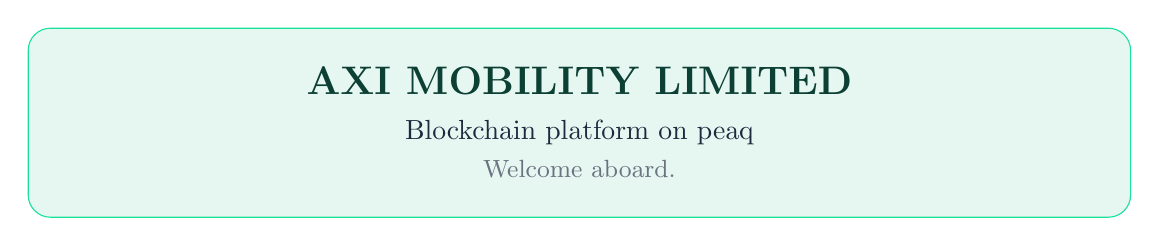
\begin{tikzpicture}
  \node[draw=axiaccent, fill=axilight, rounded corners=8pt, minimum width=14cm, minimum height=2.4cm, align=center] {
    {\Large\bfseries\color{axiprimary} AXI MOBILITY LIMITED}\\[4pt]
    {\normalsize\color{axidark} Blockchain platform on peaq}\\[2pt]
    {\small\color{axigray} Welcome aboard.}
  };
\end{tikzpicture}
\end{center}

\vfill

\begin{center}
\begin{tabular}{p{4.5cm} p{9.5cm}}
\textbf{\color{axidark}Audience:} & New blockchain developer (Solidity + Foundry background) \\
\textbf{\color{axidark}Read time:} & 60 minutes end-to-end; reference forever \\
\textbf{\color{axidark}Repo:} & \href{https://github.com/aximobility/peaq-contracts}{github.com/aximobility/peaq-contracts} \\
\textbf{\color{axidark}Sibling repo:} & \href{https://github.com/aximobility/peaq-integration}{github.com/aximobility/peaq-integration} \\
\textbf{\color{axidark}Document version:} & 1.0 \\
\textbf{\color{axidark}Date:} & May 7, 2026 \\
\textbf{\color{axidark}Reference:} & AXI/2026/ONBOARD/001 \\
\end{tabular}
\end{center}

\vspace{0.6cm}

\begin{center}
{\small\color{axigray} Apache-2.0 open source}
\end{center}

\newpage

% ============================================================
% TL;DR
% ============================================================
\section{TL;DR}

This repo holds three Solidity contracts that AXI Mobility deploys on the \textbf{peaq} blockchain.

\begin{itemize}[leftmargin=*]
  \item \textbf{InsuranceRiskOracle} --- publishes a risk score per vehicle so insurers can read it directly from the chain.
  \item \textbf{HighRiskCommandVault} --- multi-person approval gate for fleet-wide actions ("lock 47 bikes" needs 2 of 3 sign-offs).
  \item \textbf{CredentialRevocationRegistry} --- anyone can check on-chain whether a driver's licence or inspection certificate is still valid.
\end{itemize}

Plus the runbooks, threat models, and CI to ship them safely.

The repo's sibling is \texttt{peaq-integration} --- the TypeScript SDK and CLI that talks to these contracts (and to peaq's identity / role / storage pallets). Read that one second.

\begin{infobox}[title=Assumptions]
You know Solidity, have used Foundry before, and are comfortable on Linux / macOS / Windows-with-WSL. If you don't know peaq, that's fine --- we explain what's peaq-specific as we go.
\end{infobox}

% ============================================================
% REPO TOUR
% ============================================================
\section{60-second repo tour}

\begin{codebox}
peaq-contracts/\\
\textbar---- src/                       \textcolor{axigray}{<- the 3 Solidity contracts + interfaces}\\
\textbar---- test/                      \textcolor{axigray}{<- Foundry tests, one .t.sol per contract}\\
\textbar---- script/                    \textcolor{axigray}{<- Deploy + Verify forge scripts}\\
\textbar---- threat-models/             \textcolor{axigray}{<- per-contract STRIDE security analysis}\\
\textbar---- broadcast/                 \textcolor{axigray}{<- forge's deploy artifacts (auto-generated)}\\
\textbar---- lib/                       \textcolor{axigray}{<- vendored deps (forge-std, OZ) via submodules}\\
\textbar---- docs/                      \textcolor{axigray}{<- LaTeX milestone PDF + branding assets}\\
\textbar---- .github/workflows/         \textcolor{axigray}{<- CI: build, test, fmt, lint}\\
\textbar---- foundry.toml               \textcolor{axigray}{<- compiler + optimizer + remappings}\\
\textbar---- Makefile                   \textcolor{axigray}{<- one command per common task}\\
\textbar---- README.md                  \textcolor{axigray}{<- project front door}\\
\textbar---- ONBOARDING.md              \textcolor{axigray}{<- the markdown twin of this PDF}\\
\textbar---- PEAQ\_REVIEW.md             \textcolor{axigray}{<- partnership review packet for peaq}\\
\textbar---- MILESTONES.md              \textcolor{axigray}{<- what we've shipped + what's next}\\
\textbar---- AUDIT\_CHECKLIST.md         \textcolor{axigray}{<- pre-audit hardening (about 80\% closed)}\\
\textbar---- AGUNG\_DEPLOY.md            \textcolor{axigray}{<- 25-minute deploy walkthrough}\\
\textbar---- SECURITY.md                \textcolor{axigray}{<- responsible disclosure policy}\\
\textbar---- LICENSE                    \textcolor{axigray}{<- Apache-2.0}
\end{codebox}

% ============================================================
% THE THREE CONTRACTS
% ============================================================
\newpage
\section{What the three contracts do (and why they exist)}

\subsection{InsuranceRiskOracle}

\subsubsection{The problem}
Kenyan insurers price fleet premiums on patchy data, so they add a 15-25\% "uncertainty surcharge" they can't justify. Our pilot customer (ROAM Electric, 10 EV motorcycles) overpays.

\subsubsection{What this contract does}
AXI's signers post a risk score (0-1000) on-chain for each vehicle. The score is append-only and signed. Insurers read \texttt{riskScore(vehicleDid)} directly from the chain when quoting. No middleman, no API outage, no trust in AXI's database.

\subsubsection{Why on-chain}
Insurers won't trust AXI's database --- we have a financial incentive to lie. They'll trust a public log they can read and audit themselves.

\subsubsection{Key API}
\begin{itemize}[leftmargin=*, nosep]
  \item \texttt{attest(vehicleDid, score, anchorRoot, sampleSizeKm)} --- only \texttt{ATTESTOR\_ROLE} can call.
  \item \texttt{riskScore(vehicleDid)} returns \texttt{(score, attestedAt)} --- public read; reverts if older than \texttt{maxAttestationAgeSeconds}.
  \item \texttt{priceMultiplierBps(vehicleDid)} --- turns a score into a premium multiplier (basis points, 10000 = 1.0x).
\end{itemize}

\subsection{HighRiskCommandVault}

\subsubsection{The problem}
Fleet-wide actions are dangerous. "Lock 47 bikes" is one click and historically one password. Single-sig escape hatches are how fleet platforms get held ransom.

\subsubsection{What this contract does}
Multi-person approval gate. AXI staff propose a high-risk command (lock the fleet, override every route, withdraw funds). A pre-set group of approvers must sign. Once enough approve (e.g. 2 of 3), anyone can run the command --- including a regulator if AXI staff disappear.

\subsubsection{Why on-chain}
A Slack approval can be denied later. An on-chain signed approval cannot. The audit trail is the product --- insurers and regulators want proof of governance before pricing premiums or licensing the fleet.

\begin{warningbox}[title=Why NOT upgradeable]
An upgradeable approval gate is a back door. Operators see the exact rules they're approving, and AXI cannot silently change them later. This is the only contract in the repo that is fixed forever. If we want a new gate, we deploy a new contract; consumers explicitly migrate.
\end{warningbox}

\subsubsection{Key API}
\begin{itemize}[leftmargin=*, nosep]
  \item \texttt{propose(commandType, targetDid, payloadHash, K, M, expirySeconds)} returns \texttt{commandId}
  \item \texttt{approve(commandId)}
  \item \texttt{execute(commandId, payload)} --- permissionless once K approvers signed
  \item \texttt{cancel(commandId)} --- proposer only
  \item \texttt{markExpired(commandId)} --- anyone, after expiry
\end{itemize}

\subsection{CredentialRevocationRegistry}

\subsubsection{The problem}
Driver licences, NTSA inspection certificates, and insurance binders all expire or get revoked. Today fleets find out at the roadside check (about \$300 fine + tow-truck bill). Insurers find out at claim time (about \$5,000 loss). Verification is paper-based.

\subsubsection{What this contract does}
Each credential has a unique fingerprint stored on-chain. When the issuer (NTSA, insurance, fleet manager) cancels it, they post the cancellation. Anyone --- insurer, regulator, the rider app --- can instantly check whether a credential is still valid.

\subsubsection{Key API}
\begin{itemize}[leftmargin=*, nosep]
  \item \texttt{revoke(credentialHash, reasonCode)} --- \texttt{ISSUER\_ROLE} only.
  \item \texttt{revokeBatch(credentialHashes[], reasonCode)} --- capped at 100 per call (\texttt{MAX\_BATCH\_SIZE}).
  \item \texttt{unrevoke(credentialHash)} --- admin-only emergency undo.
  \item \texttt{isRevoked(credentialHash)} returns bool --- free public read.
  \item \texttt{whyRevoked(credentialHash)} returns \texttt{RevocationRecord} (reason + revoker + timestamp).
\end{itemize}

% ============================================================
% FILE-BY-FILE
% ============================================================
\newpage
\section{File-by-file walkthrough}

\subsection{Top-level config}

\begin{center}
\begin{tabular}{p{3.6cm} p{12cm}}
\toprule
{\bfseries\color{axiprimary}File} & {\bfseries\color{axiprimary}What it does} \\
\midrule
\texttt{foundry.toml} & Foundry config. Solidity 0.8.24, optimizer 10000 runs, via-IR enabled, fuzz at 256 runs. Don't downgrade --- gas measurements in \texttt{.gas-snapshot} assume them. \\
\addlinespace[2pt]
\texttt{remappings.txt} & Maps \texttt{@openzeppelin/...} and \texttt{forge-std/...} to the \texttt{lib/} submodules. \\
\addlinespace[2pt]
\texttt{foundry.lock} & Pins the Foundry toolchain version so CI and local runs match. \\
\addlinespace[2pt]
\texttt{.gitmodules} & Tracks the OpenZeppelin v5 + forge-std submodules under \texttt{lib/}. \\
\addlinespace[2pt]
\texttt{.gas-snapshot} & Committed gas-cost baseline. CI compares against this; a regression fails the build. \\
\addlinespace[2pt]
\texttt{.env.example} & Template for the env vars the deploy script needs. Never commit \texttt{.env}. \\
\addlinespace[2pt]
\texttt{.gitignore} & Ignores \texttt{out/}, \texttt{cache/}, \texttt{.env}, \texttt{node\_modules}, LaTeX artifacts. \\
\addlinespace[2pt]
\texttt{Makefile} & Single source of truth for common tasks. Every target maps to one Foundry command. \\
\addlinespace[2pt]
\texttt{LICENSE} & Apache-2.0. Permissive, commercial-friendly. \\
\bottomrule
\end{tabular}
\end{center}

\subsection{src/ --- the contracts}

\begin{center}
\begin{tabular}{p{4.5cm} p{11cm}}
\toprule
{\bfseries\color{axiprimary}File} & {\bfseries\color{axiprimary}What it does} \\
\midrule
\texttt{InsuranceRiskOracle.sol} & UUPS proxy + AccessControl + Pausable. Append-only score history per \texttt{vehicleDid}. Linear-interpolation premium multiplier between a configurable \texttt{floorBps} and \texttt{ceilingBps}. Admin can recalibrate the curve and adjust the staleness window. \\
\addlinespace[2pt]
\texttt{HighRiskCommandVault.sol} & \textbf{Not upgradeable.} AccessControl + ReentrancyGuard + Pausable. State machine: Proposed $\rightarrow$ Approved $\rightarrow$ Executed. \texttt{commandId} derivation includes \texttt{block.timestamp} + \texttt{msg.sender} to make replay safe. \\
\addlinespace[2pt]
\texttt{CredentialRevocationRegistry.sol} & UUPS proxy + AccessControl + Pausable. Append-only revocation map. \texttt{revokeBatch} is capped at \texttt{MAX\_BATCH\_SIZE = 100} to prevent gas-bomb DoS via a compromised issuer key. \\
\bottomrule
\end{tabular}
\end{center}

\subsection{src/interfaces/ --- separated interfaces}

Every contract has its public surface (events, errors, structs, function signatures) declared in a separate \texttt{I<Name>.sol} file. The implementation imports the interface and uses \texttt{override} on each public function.

\textbf{Why separated.} Three reasons:

\begin{enumerate}[leftmargin=*, nosep]
  \item SDK clients (in \texttt{peaq-integration}) consume just the interface, not the implementation. Smaller bytecode footprint, cleaner ABI export.
  \item UUPS upgrades let us change the implementation. The interface is the stable contract with consumers.
  \item Custom errors live at the interface level so external callers can decode them without the implementation source.
\end{enumerate}

\subsection{test/ --- Foundry tests}

\begin{center}
\begin{tabular}{p{5cm} p{10.5cm}}
\toprule
{\bfseries\color{axiprimary}File} & {\bfseries\color{axiprimary}What it does} \\
\midrule
\texttt{CredentialRevocationRegistry.t.sol} & 16 tests: happy paths, reverts, role-gating, batch limits, idempotency. \\
\addlinespace[2pt]
\texttt{HighRiskCommandVault.t.sol} & 18 tests: state-machine paths, replay-safety, K-of-M counting, executor permissionlessness, pause behaviour. \\
\addlinespace[2pt]
\texttt{InsuranceRiskOracle.t.sol} & 17 tests including 4 fuzz suites (256 runs each): score range, multiplier monotonicity, staleness gate, recalibration. \\
\bottomrule
\end{tabular}
\end{center}

\textbf{51 tests total. They all pass.} Run \texttt{forge test} locally before any commit.

Patterns we use everywhere:

\begin{itemize}[leftmargin=*, nosep]
  \item \texttt{vm.expectEmit(true, true, true, true)} before each event-emitting call.
  \item One \texttt{Reject*} test per custom error.
  \item Fuzz with \texttt{bound()} to keep inputs in valid ranges.
  \item \texttt{vm.startPrank(addr)} / \texttt{vm.stopPrank()} for role-based tests.
\end{itemize}

\subsection{script/ --- Foundry deploy scripts}

\begin{center}
\begin{tabular}{p{3cm} p{12.5cm}}
\toprule
{\bfseries\color{axiprimary}File} & {\bfseries\color{axiprimary}What it does} \\
\midrule
\texttt{Deploy.s.sol} & Deploys all three contracts (impl + UUPS proxy for Oracle and Registry; Vault directly). Reads admin + initial role lists from env vars. \\
\addlinespace[2pt]
\texttt{Verify.s.sol} & Verifies bytecode + initial state on a target chain after deploy. \\
\bottomrule
\end{tabular}
\end{center}

\begin{notebox}[title=Heads-up]
\texttt{broadcast/Deploy.s.sol/9990/run-latest.json} is currently a local Anvil fork run (deployer is the Anvil default \texttt{0xf39fd6...}). A real Agung deploy with a funded EOA is the next step before mainnet. We say so plainly in \texttt{PEAQ\_REVIEW.md} and the milestone PDF.
\end{notebox}

\subsection{threat-models/ --- STRIDE security analysis}

One STRIDE doc per contract. Each lists the threat surface (Spoofing / Tampering / Repudiation / Info disclosure / DoS / Elevation), the mitigation, a DREAD score, and the invariants we want an external audit firm to formally verify.

These are required pre-audit reading. \textbf{If you change a contract, update its threat model in the same PR.}

\subsection{Other top-level docs}

\begin{center}
\begin{tabular}{p{3.8cm} p{11.7cm}}
\toprule
{\bfseries\color{axiprimary}File} & {\bfseries\color{axiprimary}What it is} \\
\midrule
\texttt{README.md} & The project front door. Plain-language overview for someone who lands on the GitHub page. \\
\addlinespace[2pt]
\texttt{PEAQ\_REVIEW.md} & Partnership-facing technical review packet for peaq's tech team. 13 sections. \\
\addlinespace[2pt]
\texttt{MILESTONES.md} & What we've shipped, when, and what's next. The Markdown twin of the milestone PDF. \\
\addlinespace[2pt]
\texttt{AUDIT\_CHECKLIST.md} & Pre-audit hardening status, about 80\% complete. Auditor reads this first. \\
\addlinespace[2pt]
\texttt{AGUNG\_DEPLOY.md} & 25-minute zero-to-first-attestation deploy walkthrough. \\
\addlinespace[2pt]
\texttt{SECURITY.md} & Responsible disclosure policy. Where to send vuln reports + bounty terms. \\
\bottomrule
\end{tabular}
\end{center}

% ============================================================
% DECISIONS
% ============================================================
\newpage
\section{Why we made the decisions we did}

\subsection{Why peaq, not Ethereum / Polygon / Arbitrum}

peaq ships three things we'd otherwise have to build and maintain ourselves:

\begin{enumerate}[leftmargin=*, nosep]
  \item \textbf{\texttt{peaqDid} pallet} --- built-in identity registry. Generic L1s force you to write your own DID method + registry contract.
  \item \textbf{\texttt{peaqRbac} pallet} --- built-in role system. Generic L1s force you to write a permissions contract.
  \item \textbf{\texttt{peaqStorage} pallet} --- built-in evidence storage. Generic L1s force you to pick one model or run two chains.
\end{enumerate}

Plus peaq is mobility-native (DePIN focus) --- the ecosystem peers are ROAM-class, not generic DeFi.

We post a daily Merkle anchor to \textbf{Polygon mainnet} as a fallback in case peaq has an outage. Polygon is redundancy, not primary. peaq is the chain.

\subsection{Why UUPS for Oracle + Registry, but NOT for Vault}

\textbf{Oracle and Registry need to evolve.} We'll add features (per-issuer scope, dispute mechanism, finer score granularity) over time. UUPS lets us upgrade without breaking integrators.

\textbf{Vault must NOT evolve.} It's an approval gate. If AXI can change the rules silently, the gate is a security theatre. So Vault is fixed forever.

\textbf{Storage gap reserves.} Both UUPS contracts have \texttt{\_\_gap[N]} arrays at the end. This reserves storage slots so future upgrades can add state variables without colliding with parent-contract slots. Standard OpenZeppelin v5 pattern.

\subsection{Why role-based access (and NOT per-issuer scope on Registry, today)}

The Registry uses \texttt{ISSUER\_ROLE} --- any address with that role can revoke any credential. The on-chain \texttt{revokedBy} field records who did it.

\textbf{Why not per-credential issuer scope yet.} It's a structural change (track issuer at registration time, restrict revoke to that issuer). We'll ship it as a Phase-5 enhancement once the audit lands. Adding it under time pressure risks a real security bug. We'd rather be honest in the docs than fake the scope.

\subsection{Why custom errors instead of require strings}

Custom errors cost less gas to revert with, and they let the SDK match exact failure modes via \texttt{decodeErrorResult}. \texttt{require("not authorized")} is lazy and unscoped. We don't use \texttt{require} strings anywhere.

\subsection{Why Foundry over Hardhat}

\begin{itemize}[leftmargin=*, nosep]
  \item Solidity-native test DSL (no JS context-switching).
  \item Fuzzing is built-in.
  \item 10x faster on a cold cache.
  \item Forge scripts beat Hardhat tasks for deploys.
\end{itemize}

\subsection{Why \texttt{MAX\_BATCH\_SIZE = 100} on Registry}

A compromised \texttt{ISSUER\_ROLE} key could submit a single jumbo \texttt{revokeBatch} call to grief the chain. 100 is well below any reasonable gas limit and gives operators room to rotate keys + sweep batches over multiple blocks. The cap is enforced \textbf{on-chain} via \texttt{BatchTooLarge} --- not just documented.

\subsection{Why local Anvil fork before real Agung}

We exercise the full deploy script + initial state seeding against a fork of Agung in CI. That catches typos in the script, bad role assignments, and gas surprises before we burn real testnet tokens. The artifact in \texttt{broadcast/.../9990/run-latest.json} is that fork run.

\subsection{Why Apache-2.0}

Permissive, commercial-friendly, well-understood. The contracts have no novel cryptography or trade secrets --- public review (Linus's Law) helps us catch bugs faster than secrecy ever would.

\subsection{Why STRIDE per contract (not one global threat model)}

Each contract has different attack surface, different roles, different invariants. A global threat model collapses meaningful distinctions. Per-contract STRIDE is what audit firms expect to receive --- they can read straight from our doc into their report template.

% ============================================================
% HOW TO RUN
% ============================================================
\newpage
\section{How to run things}

\subsection{One-time setup}

\begin{codebox}
git clone git@github.com:aximobility/peaq-contracts.git\\
cd peaq-contracts\\
make install            \# installs Foundry deps via submodules\\
cp .env.example .env    \# then fill in PRIVATE\_KEY, RPC\_URL, etc.
\end{codebox}

\subsection{Daily loop}

\begin{codebox}
make build              \# forge build\\
make test               \# forge test (51 tests)\\
make fmt                \# forge fmt\\
make snapshot           \# update .gas-snapshot\\
make slither            \# local security scan (advisory)
\end{codebox}

\subsection{Before opening a PR}

\begin{codebox}
make test               \# green\\
make fmt                \# no diff\\
make snapshot           \# no unintended gas regressions
\end{codebox}

\subsection{Deploy to Agung (real, when funded)}

\begin{codebox}
make deploy-agung       \# see AGUNG\_DEPLOY.md for full walkthrough\\
make verify-agung       \# post-deploy state verification
\end{codebox}

% ============================================================
% WHERE TO LOOK
% ============================================================
\section{Where to look for what}

\begin{center}
\begin{tabular}{p{6cm} p{9.5cm}}
\toprule
{\bfseries\color{axiprimary}You want to...} & {\bfseries\color{axiprimary}Read} \\
\midrule
Understand a contract's API & \texttt{src/interfaces/I<Name>.sol} \\
\addlinespace[2pt]
See an actual scenario & \texttt{MILESTONES.md} \S 2 (Mary Akinyi, Wanjiku NTSA, etc.) \\
\addlinespace[2pt]
Run the deploy & \texttt{AGUNG\_DEPLOY.md} \\
\addlinespace[2pt]
Add a feature & \texttt{src/<Name>.sol} + matching \texttt{test/<Name>.t.sol} + update \texttt{threat-models/<Name>.STRIDE.md} \\
\addlinespace[2pt]
Audit the security model & \texttt{threat-models/} \\
\addlinespace[2pt]
Send something to peaq's team & \texttt{PEAQ\_REVIEW.md} + \texttt{docs/latex/AXI\_peaq\_Milestone\_Update.pdf} \\
\addlinespace[2pt]
Report a vuln & \texttt{SECURITY.md} \\
\addlinespace[2pt]
Track what's left & \texttt{AUDIT\_CHECKLIST.md} \\
\bottomrule
\end{tabular}
\end{center}

% ============================================================
% HOW TO CONTRIBUTE
% ============================================================
\section{How to contribute}

\begin{enumerate}[leftmargin=*]
  \item \textbf{Pick a task} from \texttt{AUDIT\_CHECKLIST.md} (the unchecked items) or an open GitHub issue.
  \item \textbf{Branch} from \texttt{main} --- \texttt{git checkout -b feat/short-name} or \texttt{fix/short-name}.
  \item \textbf{Write the test first} in \texttt{test/<Name>.t.sol}. It should fail.
  \item \textbf{Make it pass} by editing \texttt{src/<Name>.sol}.
  \item \textbf{Update the threat model} in \texttt{threat-models/<Name>.STRIDE.md} if the change touches access control, state, or external surface.
  \item \textbf{Run} \texttt{make test \&\& make fmt \&\& make snapshot} before committing.
  \item \textbf{Open the PR.} CI runs the same checks. Brian reviews.
\end{enumerate}

% ============================================================
% THINGS TO NEVER DO
% ============================================================
\section{Things to never do}

\begin{warningbox}[title=Hard rules]
\begin{itemize}[leftmargin=*, nosep]
  \item \textbf{Never} commit a \texttt{.env} file. The \texttt{.gitignore} will help; double-check before pushing.
  \item \textbf{Never} add a \texttt{require} with a string message. Use a custom error.
  \item \textbf{Never} call \texttt{delegatecall} to a user-supplied address. Ever.
  \item \textbf{Never} add an \texttt{\_authorizeUpgrade} that's not gated by \texttt{UPGRADER\_ROLE}.
  \item \textbf{Never} assume \texttt{tx.origin} for auth. Use \texttt{msg.sender}.
  \item \textbf{Never} rely on \texttt{block.timestamp} for randomness or for windows shorter than \textasciitilde 30 seconds.
  \item \textbf{Never} add a function to the Vault contract. It's frozen by design.
  \item \textbf{Never} push to \texttt{main} directly. Always via PR.
  \item \textbf{Never} force-push to \texttt{main} or any shared branch.
\end{itemize}
\end{warningbox}

% ============================================================
% WHO TO ASK
% ============================================================
\section{Who to ask}

\begin{center}
\begin{tabular}{p{4cm} p{11.5cm}}
\toprule
{\bfseries\color{axiprimary}Person} & {\bfseries\color{axiprimary}Ask them about} \\
\midrule
Brian Mwai (Founder) & peaq partnership, grant milestones, business context \\
\addlinespace[2pt]
Rhyl Kiio (CTO) & overall architecture, integration boundaries, hiring \\
\addlinespace[2pt]
Bleyle (Blockchain) & primary contact for peaq grant tech, daily anchor service, DID method \\
\addlinespace[2pt]
You & own this repo's day-to-day evolution. Ship. \\
\bottomrule
\end{tabular}
\end{center}

% ============================================================
% ROADMAP
% ============================================================
\section{What's next on the roadmap}

Pulled from \texttt{MILESTONES.md}:

\begin{enumerate}[leftmargin=*]
  \item \textbf{Real Agung deploy} with a funded EOA + multi-sig admin.
  \item Internal pilot launch (10 ROAM bikes) --- first daily anchor, first risk attestation, first revocation on real network.
  \item \textbf{External audit firm engagement} (preference among Trail of Bits, OpenZeppelin, Halborn, Sigma Prime, pending peaq's recommendation).
  \item Audit + remediation; tag \texttt{audit-v1}.
  \item \textbf{Mainnet promote} with Safe 4-of-7 multi-sig admin.
  \item Bug bounty live.
\end{enumerate}

\vspace{0.6cm}

\begin{successbox}[title=Welcome aboard]
Open a PR when you've made your first change --- even if it's just a typo fix in this doc. We work in the open.
\end{successbox}

% ============================================================
% DOC INFO
% ============================================================
\newpage
\section*{\color{axiprimary}Document info}
\addcontentsline{toc}{section}{Document info}

\vspace{0.4cm}


\begin{tikzpicture}
  \draw[axiaccent, line width=1.5pt] (0,0) -- (\textwidth-2pt,0);
\end{tikzpicture}

\vspace{0.6cm}

\begin{tabular}{p{4.5cm} p{11.5cm}}
\textbf{\color{axiprimary}Document version:} & 1.0 \\
\textbf{\color{axiprimary}Date:} & May 7, 2026 \\
\textbf{\color{axiprimary}Reference:} & AXI/2026/ONBOARD/001 \\
\textbf{\color{axiprimary}Audience:} & New blockchain developer joining AXI Mobility \\
\textbf{\color{axiprimary}Markdown twin:} & \texttt{ONBOARDING.md} in repo root \\
\textbf{\color{axiprimary}Repo:} & \href{https://github.com/aximobility/peaq-contracts}{github.com/aximobility/peaq-contracts} \\
\textbf{\color{axiprimary}Contact:} & \href{mailto:team@aximobility.com}{team@aximobility.com} \\
\textbf{\color{axiprimary}Website:} & \href{https://www.aximobility.com}{www.aximobility.com} \\
\end{tabular}

\vspace{0.8cm}

\begin{center}

\begin{tikzpicture}
  \node[draw=axiaccent, fill=axilight, rounded corners=4pt, minimum width=10cm, minimum height=1.6cm, align=center] {
    {\bfseries\color{axiprimary}AXI MOBILITY LIMITED}\\[2pt]
    {\small\color{axidark}Nation Centre, Kimathi Street \enspace$\cdot$\enspace P.O.\ Box 49010, G.P.O.\ Nairobi}\\[2pt]
    {\small\color{axigray}+254 105 675 224 \enspace$\cdot$\enspace \href{https://www.aximobility.com}{www.aximobility.com}}
  };
\end{tikzpicture}
\end{center}

\end{document}
